%% abtex2-modelo-trabalho-academico.tex, v-1.4 laurocesar
%% Copyright 2012-2013 by abnTeX2 group at http://abntex2.googlecode.com/ 
%%
%% This work may be distributed and/or modified under the
%% conditions of the LaTeX Project Public License, either version 1.3
%% of this license or (at your option) any later version.
%% The latest version of this license is in
%%   http://www.latex-project.org/lppl.txt
%% and version 1.3 or later is part of all distributions of LaTeX
%% version 2005/12/01 or later.
%%
%% This work has the LPPL maintenance status `maintained'.
%% 
%% The Current Maintainer of this work is the abnTeX2 team, led
%% by Lauro César Araujo. Further information are available on 
%% http://abntex2.googlecode.com/
%%
%% This work consists of the files abntex2-modelo-trabalho-academico.tex,
%% abntex2-modelo-include-comandos and abntex2-modelo-references.bib
%%

% ------------------------------------------------------------------------
% ------------------------------------------------------------------------
% abnTeX2: Modelo de Trabalho Acadêmico (tese de doutorado, dissertação de
% mestrado e trabalhos monográficos em geral) em conformidade com 
% ABNT NBR 14724:2011: Informação e documentação - Trabalhos acadêmicos -
% Apresentação
% ------------------------------------------------------------------------
% ------------------------------------------------------------------------

\documentclass[12pt,openright,twoside,a4paper]{abntex2}	% frente e verso
%\documentclass[article,11pt,oneside,a4paper]{abntex2}	
%\documentclass[12pt,oneside,a4paper]{abntex2}			% apenas frente

% ---
% PACOTES
% ---

% ---
% Pacotes fundamentais 
% ---

\usepackage{abntex2-ufc}
\usepackage{cmap}			% Mapear caracteres especiais no PDF
\usepackage{multirow}	
%\usepackage{fontspec}			% Pacote para utilizar OpenType fonts in Latex.
%\setmainfont{Times New Roman}		% Define a Fonte, mas precisa do "xelatex"~ or~ "lualatex".


\usepackage{lmodern}			% Usa a fonte Latin Modern
\usepackage[T1]{fontenc}		% Seleção de códigos de fonte.

\usepackage[utf8]{inputenc}		% Determina a codificação utilizada (conversão automática dos acentos)
\usepackage{makeidx}    	        % Cria o indice
\usepackage{hyperref}  			% Controla a formação do índice
\usepackage{lastpage}			% Usado pela Ficha catalográfica
\usepackage{indentfirst}		% Indenta o primeiro parágrafo de cada seção.
\usepackage{nomencl} 			% Lista de simbolos
\usepackage{color}			% Controle das cores


\usepackage{algpseudocode}
\usepackage{algorithm}
% sem todo
%\usepackage[disable]{todonotes}
% com todo
\usepackage{todonotes}
\usepackage[none]{hyphenat}
\usepackage{array}
\usepackage{float}
\restylefloat{table}

\usepackage{graphicx}			% Inclusão de gráficos
\usepackage{epstopdf}
\usepackage{subfig}

\DeclareGraphicsExtensions{.pdf,.png,.jpg} % Declara as extensões para Graphics

% pacotes para utilização de matemática
\usepackage{amsfonts}
\usepackage{amssymb}
\usepackage{amsthm}
\usepackage{amsmath}

%% pacotes para o cronograma
\usepackage{colortbl}
\usepackage{booktabs}
\definecolor{tcA}{gray}{0}


\usepackage{pdfpages}

% ---
	
% ---
% Pacotes de citações
% ---
%\usepackage[brazilian,hyperpageref]{backref} % Paginas com as citações na bibl
\usepackage[alf]{abntex2cite} % Citações padrão ABNT

% ==================== Definições de conveniência =================

\newcommand{\norma}[1]{\left|\left|#1\right|\right|}
\newtheorem{Def}{Definição}

% --- 
% CONFIGURAÇÕES DE PACOTES
% --- 

% ---
% Configurações do pacote backref
% Usado sem a opção hyperpageref de backref
%\renewcommand{\backrefpagesname}{Citado na(s) página(s):~}
% Texto padrão antes do número das páginas
%\renewcommand{\backref}{}
% Define os textos da citação
%\renewcommand*{\backrefalt}[4]{
%	\ifcase #1 %
%		Nenhuma citação no texto.%
%	\or
%		Citado na página #2.%
%	\else
%		Citado #1 vezes nas páginas #2.%
%	\fi}%
% ---

% ---
% Informações de dados para CAPA e FOLHA DE ROSTO
% ---
\titulo{Aplicação de aprendizado de máquina ao problema de evasão de discentes da UFC}
\autor{Abelardo Vieira Mota}
\local{Fortaleza}
\data{2015}
\orientador{João Paulo Pordeus Gomes}
\instituicao{%
  Universidade Federal do Ceará
  \par
  Centro de Ciências 
  \par
  Departamento de Computação
  \par
  Programa de Pós-Graduação em Ciência da Computação}
\tipotrabalho{Dissertação (Mestrado)}
% O preambulo deve conter o tipo do trabalho, o objetivo, 
% o nome da instituição e a área de concentração 
%\preambulo{Modelo canônico de trabalho monográfico acadêmico em conformidade com as normas ABNT apresentado à comunidade de usuários \LaTeX.}
% ---
% ---
% Configurações de aparência do PDF final

% alterando o aspecto da cor azul
\definecolor{blue}{RGB}{41,5,195}

%\captionsetup{%
  %singlelinecheck=false,
  %tableposition=left
%}

% informações do PDF
\hypersetup{
     	%backref=true,
     	%pagebackref=true,
		%bookmarks=true,         		% show bookmarks bar?
		pdftitle={\imprimirtitulo}, 
		pdfauthor={\imprimirautor},
    	pdfsubject={\imprimirpreambulo},
		pdfkeywords={PALAVRAS}{CHAVES}{abnt}{abntex}{abntex2},
	    pdfproducer={LaTeX with abnTeX2}, 	% producer of the document
	    pdfcreator={\imprimirautor},
    	colorlinks=true,       		% false: boxed links; true: colored links
    	linkcolor=blue,          	% color of internal links
    	citecolor=blue,        		% color of links to bibliography
    	filecolor=magenta,      		% color of file links
		urlcolor=blue,
		bookmarksdepth=4
}
% --- 

% --- 
% Espaçamentos entre linhas e parágrafos 
% --- 

% O tamanho do parágrafo é dado por:
\setlength{\parindent}{1.3cm}

% Controle do espaçamento entre um parágrafo e outro:
\setlength{\parskip}{0.2cm}  % tente também \onelineskip



% Controles do espaçamento entre linhas:
%\OnehalfSpacing	% espaçamento um e meio (padrão); 
%\DoubleSpacing		% espaçamento duplo
\SingleSpacing		% espaçamento simples	
% --- 
	

% ---
% compila o indice
% ---
\makeindex
% ---

% ---
% Compila a lista de abreviaturas e siglas
% ---
% \makenomenclature
% ---

% ----
% Início do documento
% ----
\begin{document}


% ----------------------------------------------------------
% ELEMENTOS PRÉ-TEXTUAIS
% ----------------------------------------------------------

%% ----------------------------------------------------------
% ELEMENTOS PRÉ-TEXTUAIS
% ----------------------------------------------------------
% \pretextual

% ---
% Capa
% ---
\imprimircapa

% ---
% Folha de rosto
% (o * indica que haverá a ficha bibliográfica)

% \imprimirfolhaderosto

% ---
%\imprimirfolhaderosto*

% ---

% ---
% Inserir a ficha bibliografica
% ---

% Isto é um exemplo de Ficha Catalográfica, ou ``Dados internacionais de
% catalogação-na-publicação''. Você pode utilizar este modelo como referência. 
% Porém, provavelmente a biblioteca da sua universidade lhe fornecerá um PDF
% com a ficha catalográfica definitiva após a defesa do trabalho. Quando estiver
% com o documento, salve-o como PDF no diretório do seu projeto e substitua todo
% o conteúdo de implementação deste arquivo pelo comando abaixo:
%
% \begin{fichacatalografica}
%     \includepdf{fig_ficha_catalografica.pdf}
% \end{fichacatalografica}
%\begin{fichacatalografica}
%	\vspace*{\fill}					% Posição vertical
%	\hrule							% Linha horizontal
%	\begin{center}					% Minipage Centralizado
%	\begin{minipage}[c]{12.5cm}		% Largura
%	
%	\imprimirautor
%	
%	\hspace{0.5cm} \imprimirtitulo  / \imprimirautor. --
%	\imprimirlocal, \imprimirdata-
%	
%	\hspace{0.5cm} \pageref{LastPage} p. : il. (algumas color.) ; 30 cm.\\
%	
%	\hspace{0.5cm} \imprimirorientadorRotulo~\imprimirorientador\\
%	
%	\hspace{0.5cm}
%	\parbox[t]{\textwidth}{\imprimirtipotrabalho~--~\imprimirinstituicao,
%	\imprimirdata.}\\
%	
%	\hspace{0.5cm}
%		1. Palavra-chave1.
%		2. Palavra-chave2.
%		I. Orientador.
%		II. Universidade xxx.
%		III. Faculdade de xxx.
%		IV. Título\\ 			
%	
%	\hspace{8.75cm} CDU 02:141:005.7\\
%	
%	\end{minipage}
%	\end{center}
%	\hrule
%\end{fichacatalografica}

% ---


% ---
% Inserir folha de aprovação
% ---

% Isto é um exemplo de Folha de aprovação, elemento obrigatório da NBR
% 14724/2011 (seção 4.2.1.3). Você pode utilizar este modelo até a aprovação
% do trabalho. Após isso, substitua todo o conteúdo deste arquivo por uma
% imagem da página assinada pela banca com o comando abaixo:
%
% \includepdf{folhadeaprovacao_final.pdf}
%

%\begin{folhadeaprovacao}
%
%  \begin{center}
%    \vspace*{1cm}
%    {\ABNTEXchapterfont\large\imprimirautor}
%
%    \vspace*{\fill}\vspace*{\fill}
%    {\ABNTEXchapterfont\bfseries\Large\imprimirtitulo}
%    \vspace*{\fill}
%    
%    \hspace{.45\textwidth}
%    \begin{minipage}{.5\textwidth}
%        \imprimirpreambulo
%    \end{minipage}%
%    \vspace*{\fill}
%   \end{center}
    
%   Trabalho aprovado. \imprimirlocal, 24 de novembro de 2012:

%   \assinatura{\textbf{\imprimirorientador} \\ Orientador} 
%   \assinatura{\textbf{Professor} \\ Convidado 1}
%   \assinatura{\textbf{Professor} \\ Convidado 2}
   %\assinatura{\textbf{Professor} \\ Convidado 3}
   %\assinatura{\textbf{Professor} \\ Convidado 4}
      
%   \begin{center}
%    \vspace*{0.5cm}
%    {\large\imprimirlocal}
%    \par
%    {\large\imprimirdata}
%    \vspace*{1cm}
%  \end{center}
  
%\end{folhadeaprovacao}

% ---

\begin{comment}
% ---
% Dedicatória
% ---
\begin{dedicatoria}
   \vspace*{\fill}
   \centering
   \noindent
   Nem terminei ainda rs\vspace*{\fill}
\end{dedicatoria}
% ---

% ---
% Agradecimentos
% ---
%\begin{agradecimentos}
%Agredicmentos..
%\end{agradecimentos}
% ---

% ---
% Epígrafe
% ---
\begin{epigrafe}
    \vspace*{\fill}
	\begin{flushright}
		\textit{``Prefiro ser \\ Essa metamorfose ambulante''} \\
		(Raul Seixas)
	\end{flushright}
\end{epigrafe}
% ---
\end{comment}

% ---
% RESUMOS
% ---

% resumo em português
\begin{abstract}
% contexto - resultado - conclusão

A evasão de discentes de cursos de ensino superior é um problema que tem recebido atenção do governo federal, dadas as altas taxas observadas nos últimos anos e por implicar em desperdício de recursos e de tempo. Esse problema tem sido objeto de estudos que buscam identificar suas causas e construir modelos de predição que possam ser utilizados para identificar discentes com grande probabilidade de abandonarem seus cursos, de forma que ações possam ser executadas a fim de diminuir essa probabilidade. Uma das ferramentas utilizadas ultimamente para construção desses modelos é Aprendizado de Máquina, subárea de Inteligência Artificial composta por algoritmos e técnicas que permitem que um programa melhore sua performance a partir de dados. Este trabalho objetiva avaliar a aplicabilidade de Aprendizado de Máquina ao problema de evasão de discentes da UFC.

 \vspace{\onelineskip}
    
 \noindent
 \textbf{Palavras-chaves}: Aprendizado de máquina. Evasão.
 
\end{abstract}

% resumo em inglês
\begin{resumo}[Abstract]
The ideal abstract will be brief, limited to one paragraph and no more than six ou seven sentences, to let readers scan it quickly for an overview of the paper's content.
 \vspace{\onelineskip}

 \noindent 
 \textbf{Key-words}: Machine Learning. Drop-out.
\end{resumo}

% ---
% inserir lista de ilustrações
% ---
\pdfbookmark[0]{\listfigurename}{lof}
\listoffigures*
\cleardoublepage
% ---

% ---
% inserir lista de tabelas
% ---
\pdfbookmark[0]{\listtablename}{lot}
\listoftables*
\cleardoublepage
% ---

% ---
% inserir lista de abreviaturas e siglas
% A lista de Abreviaturas e Siglas pode ser facilmente montada com o pacote 
% nomencl. Abaixo segue um exemplo.
% ---
\nomenclature{Fig.}{Figura}
\nomenclature{$A_i$}{Area of the $i^{th}$ component} 
\nomenclature{456}{Isto é um número}
\nomenclature{123}{Isto é outro número}
\nomenclature{a}{primeira letra do alfabeto}
\nomenclature{lauro}{este é meu nome} 

\renewcommand{\nomname}{Lista de abreviaturas e siglas}
\pdfbookmark[0]{\nomname}{las}
\printnomenclature
\cleardoublepage
% ---

% ---
% inserir lista de símbolos
% ---
% O abnTeX2 não provê mecanismo para lista de símbolos.
% ---

% ---
% inserir o sumario
% ---
\pdfbookmark[0]{\contentsname}{toc}
\tableofcontents*
\cleardoublepage
% ---


% ----------------------------------------------------------
% ELEMENTOS TEXTUAIS
% ----------------------------------------------------------
% É possível usar \textual ou \mainmatter, que é a macro padrão do memoir.  

\mainmatter

%\listoftodos
%\chapter{Introdução}

% O que é o problema

% [Background]
O fenômeno evasão de discente consiste na interrupção de um processo de aprendizado de um discente antes de sua conclusão. Por exemplo, um discente que abandonou o curso de Computação, na UFC, no qual estava matriculado havia dois anos, pois precisou trabalhar para sustentar sua família e os horários das disciplinas eram incompatíveis com os horários do trabalho. Deste exemplo pode-se observar alguns dos atributos do fenômeno: o agente que interrompeu o processo, o discente, o curso, a instituição de ensino superior(IES), o tempo cursado e o motivo.

% # discutir mais sobre o fenômeno -> números no brasil, na ufc etc
% dados de qtd evasão na UFC e no Brasil

% Consequências
Sob a perspectiva de que o processo de aprendizado é um investimento e que o resultado esperado é a sua conclusão, o fenômeno evasão de discente pode ser considerado um problema: para a sociedade, com a frustração da expectativa de formação de profissionais e pesquisadores qualificados; para a instituição de ensino, caso tenha realizado investimentos em infraestrutura e em recursos humanos para atender a uma quantidade esperada de discentes ativos maior que a real, ocorrendo desperdício de recursos; caso seu orçamento seja ou função da quantidade de discentes ativos, no caso das instituições de ensino particulares, ou função da quantidade de discentes diplomados, no caso das instituições de ensino superior públicas\todo{validar o impacto da evasão no orçamento das IFES}; para o indivíduo que investiu tempo, dinheiro e dedicação, mas não terá os benefícios da conclusão da graduação, crítica no caso das profissões que exigem, para serem exercidas, diploma de graduação.

Em \cite{evasao_global} foi estimado um prejuízo econômico, decorrente da evasão de discentes de graduação no período de 2007 a 2012, para a UFPB, de R\$ 415.032.704,52. A estimativa considera perdidos os recursos financeiros investidos para manutenção do discente que não concluiu a graduação, utilizando a fórmula:

$Perda\ Anual=n\_evadidos \times t\_permanencia \times v\_aluno$

onde:
\begin{itemize}
\item $n\_evadidos$ representa a quantidade, por ano, média de discentes que evadiram no período, considerada a média aritmética do total de discentes que evadiram no período pela quantidade de anos do período.
\item $t\_permanencia$ representa o tempo de permanência esperado de um discente antes de evadir.
\item $v\_aluno$ representa o custo corrente com hospital universitário por aluno corrente, indicador definido pelo TCU\cite{indicadores_TCU}.
\end{itemize}

Aplicando a fórmula para os dados da UFC, obtemos o resultado \todo[inline]{estimar o prejuízo econômico da evasão para a UFC}.

% motivação para resolver o problema

O estudo da evasão de discentes é motivado não apenas pelos problemas que dela podem decorrer mas também por diretrizes dos diversos níveis administrativos envolvidos com o processo.

No nível federal, redução da ocorrência desse fenômeno faz parte de uma das diretrizes do Programa de Apoio a Planos de Reestruturação e Expansão das Universidades Federais(REUNI), instituído pelo Decreto nº 6.096, de 24 de abril de 2007\cite{reuni}:
\begin{quote}
I - redução das taxas de evasão, ocupação de vagas ociosas e aumento de vagas de ingresso, especialmente no período noturno;
\end{quote}

Na UFC, o instrumento de planejamento Plano de Desenvolvimento Institucional\cite{pdi_ufc}, para o período de 2013 a 2017, apresenta como um dos objetivos da política de assistência estudantil a redução da evasão; o programa de gestão da chapa eleita para reitoria no período de 2015 a 2019\cite{henry} apresenta um conjunto de propostas que possuem como um dos objetivos a redução dos índices de evasão; o planejamento estratégico do Centro de Tecnologia da UFC para o período de 2015 a 2025 propõe a criação de uma equipe de apoio pedagógico para atuar no combate a problemas relacionados à evasão de discentes.


% Soluções

Em \cite{evasao_panorama2} são apresentadas sete ações que ajudam a diminuir a ocorrência de evasão de discentes:

\begin{enumerate}

\item Estabelecer um grupo de trabalho encarregado de reduzir a evasão
\item Avaliar as estatísticas da evasão
\item Determinar as causas da evasão
\item Estimular a visão da IES centrada no aluno
\item Criar condições que atendam aos objetivos que atraíram os alunos
\item Tornar o ambiente e o trânsito na IES agradáveis aos alunos
\item Criar programa de aconselhamento e orientação dos aluno

\end{enumerate}

Estas ações podem ser beneficiadas pela utilização de ferramentas de Aprendizado de Máquina, subárea de Inteligência Artificial, que estuda o desenvolvimento de programas cujas performances melhorem a partir de dados. 

% argumentar que é um problema complexo
% tese de Tinto de que normalmente é a combinação de pequenas causas

% Predição
Para diminuir as taxas de evasão, uma das estratégias adotadas é a identificação precoce de discentes com grande tendência para abandonarem seus cursos e a execução de ações que minimizem tal tendência. A identificação pode ser conduzida por observação do comportamento e resultados dos discentes, de forma subjetiva, pelos docentes e coordenadores de cursos, por exemplo. Em estudo realizado no departamento de engenharia elétrica da Eindhoven University of Technology\cite{Predicting_Students}, é relatado que em dezembro os discentes desse departamente recebem um aviso informando se são ou não aconselhados a continuarem no curso. Esse aviso é baseado na performance do discente no curso e em informações obtidas de professores do primeiro semestre e de discentes monitores. É relatado que o aviso parece ter bastante acurácia: geralmente discentes aconselhados a continuarem têm sucesso no próximo ano do curso, enquanto aqueles desaconselhados geralmente não continuam no curso.
Dois problemas decorrem dessa forma de identificação: sendo conduzida por pessoas, essa forma de identificação é limitada pelo conjunto de observações as quais o observador tem acesso; sendo subjetiva, seus resultados podem sofrer resistência para serem aceitos. A utilização de técnicas de aprendizado de máquina como forma de identificação pode contornar esses problemas, por, primeiro, fazer uso de dados registrados por sistemas de informação, provavelmente contendo informações mais amplas que as que uma pessoa pode observar; segundo, por fazer maior uso de dados registrados, sendo aceita mais facilmente como identificação objetiva. Nesse estudo foram utilizados diversos algoritmos de aprendizado de máquina com o objetivo de tentar detectar que um estudante irá abandonar seu curso. Foram utilizadas informações de discente referentes tanto ao período anterior ao seu ingresso na universidade, quanto ao posterior.


% Objetivo

O presente trabalho objetiva avaliar a aplicabilidade de técnicas de aprendizado de máquina ao problema de evasão de discentes na UFC.
%\todo{sobre data mining - qual o super artigo básico?}
Aprendizado de máquina é uma subárea de inteligência artificial que agrupa conhecimentos sobre algoritmos e técnicas que permitam que um programa melhore sua performance a partir de dados. Mais formalmente, \cite{Tom_mitchell} define o aprendizado de um programa por\todo{como por a definition?}

Definition: A computer program is said to learn from experience E with respect to some class of tasks T and performance measure P, if its performance at tasks in T, as measured by P, improves with experience E. 

Para a aplicação dos conhecimentos de aprendizado de máquina para solucionar um problema, esses três elementos, tarefa(task), medida de performance(performance measure) e experiência(experience) devem ser identificados.
\todo{por que não aplicar outras técnicas?}
\todo{exemplos}
Reconhecimento de dígito manualmente escrito

O problema de reconhecimento de dígito manualmente escrito consiste na identificação automatizada do valor de um dígito manualmente escrito contido em uma imagem.

Tarefa: dada uma imagem contendo um dígito manualmente escrito, identificar qual o valor do dígito nela contido.
Experiência: arquivo de imagem contendo um dígito manualmente escrito e o valor do dígito nele contido.
Medida de performance: a proporção de dígitos corretamente identificados. 

Identificação de autoria de textos

O problema de identificação de autoria de textos consiste na identificação automatizada do autor de um texto.

Tarefa: dado um texto, identificar qual seu autor.
Experiência: texto e respectivo autor.
Medida de performance: a proporção de autores corretamente identificados.

\todo{problemas com tarefa, medida de performance, experiencia menos comuns}

\todo{bla bla bla de machine learning}

\todo{definição informal de aprendizado de máquina}
\todo{definição formal de aprendizado de máquina}
\todo{métricas}
\todo{algoritmos}
\todo{métodos de teste}
\todo{aplicação}
\cite{ML_debt} \cite{ML_know}
\todo{machine learning}
\bibliographystyle{plain}

%\todo{tabela com dados dos estudos analisados - ver fichamento.xlsx}
\todo{descrever, em termos gerais, cada estudo}
Em \cite{EDM_pred_dropout} são aplicados algoritmos de aprendizado de máquina a dados de estudantes do Eletrical Engineering department, Eindhoven University of Technology , com o objetivo de identificar estudantes em grupos de risco de evasão. É relatado que esse departamento já avaliava os estudantes com relação ao risco de evasão, mas de forma subjetiva. O estudo ressalta o maior custo da ocorrência de falsos negativos que de falsos positivos na identificação de estudantes com risco de evasão. Ocorre que, argumenta-se, há prejuízo maior em não oferecer apoio a um estudante com risco de evasão do que oferecer, desnecessariamente, apoio a um estudante sem tal risco. O estudo faz uso então de uma matriz de custo, com o classificador CostSensitiveClassifier, do Weka, obtendo melhores resultados, com relação a ocorrência de falsos negativos, mas com perdas de acurácia. 

\cite{EDM_review_and_soa} 
\cite{EDM_retention} 
\cite{EDM_education}
\cite{EDM_dropout_rates}
\cite{EDM_ufrj}
\cite{EDM_ufrj2}
\cite{EDM_brasil}
\chapter{Método}

\todo[inline]{O capítulo todo é um resumo do CRISP-DM 1.0... fico dando \\cite em todo parágrafo? o mesmo para o capítulo sobre aprendizado de máquina}

% Por que seguir um processo?
\todo[inline]{Por que um processo?}

% Reproducibilidade/padronização/etc
\cite{ML_know} \cite{balance-anarchy} \cite{ML_debt} \cite{replicability}

O processo de aplicação de técnicas de Mineração de Dados para atender a um problema real demanda não apenas conhecimentos e execução de atividades relacionadas, estritamente, a aprendizado de máquina, mas também conhecimentos e execução de atividades relacionadas ao entendimento do problema em questão. A fim de organizar as atividades envolvidas nesse processo, foram desenvolvidas especificações de processos que orientam quais os passos devem ser seguidos para partir do entendimento de um problema e chegar a uma solução baseada em Mineração de Dados, como o CRISP-DM, o KDD e o SEMMA\cite{CRISP-DM-KDD-SEMMA}.

% Por que CRISP-DM?
\todo{por que crisp-dm}
\cite{CRISP-DM-KDD-SEMMA}

\section{Processo CRISP-DM}

% História do CRISP-DM
%% p. 1-2
CRISP-DM(CRoss-Industry Standard Process for Data Mining) é um processo de aplicação de Mineração de Dados, desenvolvido pelo CRISP-DM Special Interest Group e publicado em 2000. Foi concebido em 1996 por três empresas que utilizavam Mineração de Dados: DaimlerChrysler(à época Daimler-Benz), SPSS(à época ISL) e NCR; motivadas pela incerteza com relação à qualidade de seus trabalhos, pelo questionamento de se toda nova empresa que quisesse aplicar Mineração de Dados \todo{falar sobre mineração de dados como super área no capítulo sobre aprendizado de máquina} teria que passar pelo aprendizado pelo qual passaram, baseado em tentativa e erro, e como garantirem, para seus clientes, que Mineração de Dados era uma área suficientemente madura para ser incorporada a seus processos de negócio. Em 1999 foi publicado um draft do CRISP-DM versão 1.0, sendo aplicado pela DaimlerChrysler, SPSS e NCR a vários tipos de aplicações, indústrias e problemas de negócio, sendo considerado, então, validado suficientemente para ser publicado e distribuído\cite{CRISP-DM}.

% Overview do CRISP-DM
%% p. 6
CRISP-DM segue uma estrutura hierárquica, composta por quatro níveis de abstração(do mais genérico ao mais específico):fase, tarefa genérica, tarefa especializada e instância de processo. Os dois primeiros níveis, fase e tarefa genérica, foram modelados a fim de serem: genéricos o suficiente para atenderem às todas aplicações de Mineração de Dados; completos, abrangendo todo o processo de Mineração de Dados; e estáveis, sendo aplicáveis tanto para as técnicas de Mineração de Dados existentes, quanto às que venham a ser desenvolvidas. O terceiro nível, tarefa especializada, é composto pelas tarefas a serem executadas em situações específicas para alcançar os objetivos das tarefas genéricas. Exemplificando, seja a tarefa genérica Limpar dados: a ela relacionadas estão as tarefas especializadas Limpar dados numéricos e Limpar dados categóricos. O quarto nível, instância de processo, é composto pelos registros de ações, decisões e resultados de uma execução do processo\cite{CRISP-DM}.

% Sobre não ser linear, mas interativo incremental
Apesar de a representação do processo sugerir que ele é composto por uma sequência fixa de fases, na prática as tarefas podem ser executadas seguindo outras ordens: é o caso de, por exemplo, na tarefa Avaliação do modelo ser verificado que são necessários mais dados, a serem adquiridos através de tarefas anteriores, de acordo com o diagrama do processo.

% Mapeamento modelo -> instância
%% p. 7-8
Para o mapeamento do modelo em uma instância do processo, a especificação do CRISP-DM identifica como relevantes quatro dimensões do contexto de Mineração de Dados: domínio de aplicação, tipo de problema de Mineração de Dados, aspectos técnicos e ferramentas e técnicas. Os valores dessas dimensões são utilizados nas decisões sobre que tarefas específicas podem ou devem ser executadas.

O processo de mapeamento do CRISP-DM a uma instância do processo é, de acordo com o CRISP-DM, composto pelas etapas:

\begin{enumerate}

\item Analisar o contexto, identificando os valores para as dimensões domínio de aplicação, tipo de problema de Mineração de Dados, aspectos técnicos e ferramentas e técnicas

\item Remover do modelo CRISP-DM os detalhes não aplicáveis ao contexto analisado

\item Adicionar detalhes específicos do contexto analisado

\item Especializar(ou instanciar) elementos genéricos do modelo de acordo com características concretas do contexto

\item Possivelmente renomear elementos genéricos do modelo a fim de tornar mais explícito seu significado, de acordo com o contexto

\end{enumerate}

\begin{figure}[H]
	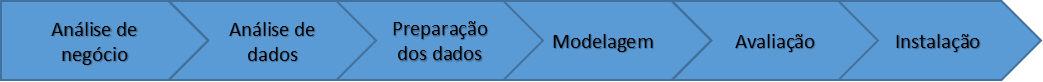
\includegraphics[scale=0.8]{img/CRISP-DM-main.png}
	\caption{Fases do CRISP-DM}
	\label{img:CRISP-DM-diagram}
\end{figure}

% Overview das fases 
%% p. 10-11
A seguir segue uma descrição breve de cada uma das fases:

\begin{enumerate}

\item \textbf{Análise do negócio}:
O objetivo desta fase é entender os requisitos e objetivos do projeto sob uma perspectiva de negócio, traduzí-los para requisitos e objetivos sob uma perspectiva de Mineração de Dados e então traçar um plano preliminar para alcançá-los.

\item \textbf{Análise dos dados}:
Esta fase inicia com uma coleta inicial de dados e segue para o estudo dos dados a fim de identificar problemas de qualidade, obter insights e detectar possíveis subconjuntos de dados que permitam desenvolver hipóteses sobre informações que não estejam presentes.

\item \textbf{Preparação dos dados}:
Esta fase é composta por atividades necessárias para gerar, a partir dos dados inicialmente coletados, um conjunto de dados a ser utilizado pelas ferramentas de modelagem. Inclui atividades como seleção de tabelas, de registros, de atributos e transformação de dados.

\item \textbf{Modelagem}:
Nesta fase são desenvolvidos e otimizados modelos. Normalmente aplicam-se ao problema mais de uma técnicas de modelagem. Como algumas técnicas de modelagem podem possuir pré requisitos sobre os dados, pode ser necessário voltar para a fase Preparação dos dados.

\item \textbf{Avaliação}:
Esta fase é iniciada quando já foi desenvolvido um modelo com alta qualidade, do ponto de vista da Mineração de Dados. Nela são avaliados a adequação do modelo como ferramenta para alcançar o objetivo de negócio que motivou o projeto e a qualidade da instância do processo. Ela termina com a decisão pela utilização ou não dos resultados obtidos.

\item \textbf{Instalação}:
Após o desenvolvimento de um modelo, faz-se necessário que ele seja disponibilizado para os usuários finais, seja na forma de relatórios, seja na forma de sistemas de apoio à tomada de decisão, para que seja efetivamente utilizado, auxiliando no alcance dos objetivos de negócio que motivaram a criação do projeto.

\end{enumerate}

A seguir segue o detalhamento de cada fase, especificando suas tarefas genéricas e os documentos que são gerados.

\newpage

\subsection*{1 - Análise do negócio}

% diagrama

\begin{figure}[H]
	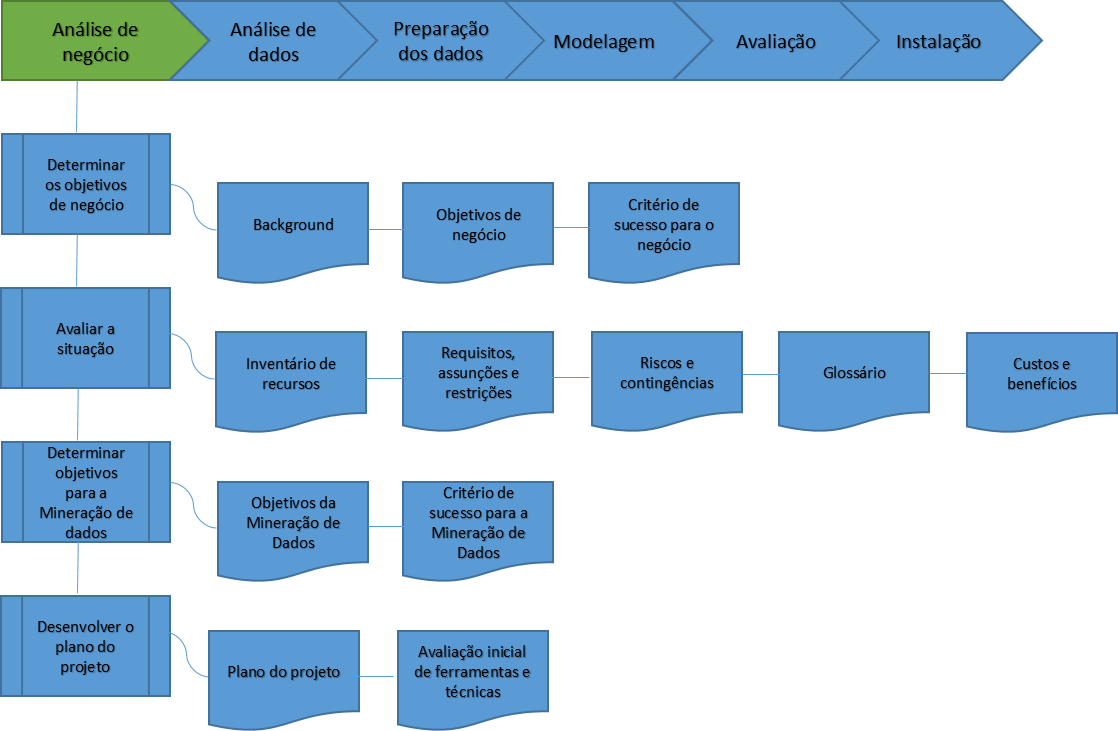
\includegraphics[scale=0.8]{img/CRISP-DM-Analise-de-negocio.png}
	\caption{Detalhamento da fase Análise de negócio}
	\label{img:CRISP-DM-analise-de-negocio}
\end{figure}

% Tarefas e saídas

\subsubsection*{\textbf{1.1 - Determinar os objetivos de negócio}}

O primeiro passo em um projeto de Mineração de Dados é analisar, sob uma perspectiva de negócio, o que o cliente deseja alcançar. Normalmente o cliente possui várias restrições e objetivos concorrentes, que devem ser balanceados. O objetivo desta tarefa é descobrir fatores importantes do negócio que possam influenciar no resultado do projeto. Uma das consequências de se negligenciar esse passo é o projeto finalizar respondendo corretamente a perguntas erradas.

\subsubsection*{Background}
\todo{esqueci de traduzir Background...}

Registro das informações levantadas sobre o estado do negócio no início do projeto.

\subsubsection*{Objetivos do negócio}

Registra os objetivos de negócio que motivaram a criação do projeto, além de questões a eles relacionadas que o cliente deseje responder. 

\subsubsection*{Critério de sucesso para o negócio}

Registra os critérios para que o projeto seja considerado um sucesso, sob uma perspectiva de negócio.

\subsubsection*{\textbf{1.2 - Avaliar a situação}}

O objetivo desta tarefa é analisar mais detalhadamente informações importantes para determinar os objetivos da Mineração de Dados e desenvolver um plano para o projeto. São analisadas informações como quais os recursos estão disponíveis, quais as restrições impostas, quais as assunções e outros fatores que forem relevantes para a especificação dos objetivos de Mineração de Dados e para o desenvolvimento do plano do projeto.

\subsubsection*{Inventário de recursos}

Registra os recursos disponíveis para o projeto, como recursos humanos(especialistas do negócio, analistas de dados, técnicos de suporte), dados(arquivos, bases de dados operacionais, data warehouses), hardwares e softwares.

\subsubsection*{Requisitos, assunções e restrições}

Registra os requisitos do projeto, incluindo prazos, níveis de qualidade, segurança e aspectos legais; as assunções do projeto, sejam assunções que poderão ser verificadas a partir dos dados utilizados pelo projeto, sejam assunções que não poderão ser verificadas, que devem ser registradas, visto que podem afetar a validade dos resultados do projeto; e as restrições do projeto, sejam restrições na disponibilidade de recursos, sejam restrições tecnológicas.

\subsubsection*{Riscos e contingências}

Registra os eventos que, caso ocorram, poderão afetar os prazos ou a qualidade do projeto, bem como os planos de contingência, detalhando que ações devem ser executadas caso esses eventos ocorram.

\subsubsection*{Glossário}

Registra o conjunto de termos e seus significados que são relevantes para o projeto. Inclui tanto termos pertencentes à terminologia do negócio, quanto termos pertencentes à terminologia de Mineração de Dados.

\subsubsection*{Custos e benefícios}

Registra uma análise dos custos do projeto comparados com os potenciais benefícios para o negócio, caso o projeto alcance sucesso. Essa comparação deve ser o mais específico possível. Por exemplo, pode-se utilizar o custo estimado do projeto e a economia esperada, em termos monetários.

\subsubsection*{\textbf{1.3 - Determinar os objetivos de Mineração de Dados}}

O objetivo desta tarefa é traduzir para objetivos de Mineração de Dados os objetivos de negócio analisados na tarefa Determinar os objetivos de negócio.

\subsubsection*{Objetivos de Mineração de Dados}

Registra os objetivos a serem alcançados pelo projeto para auxiliar no alcance dos objetivos de negócio.

\subsubsection*{Critério de sucesso para a Mineração de Dados}

Registra, em termos técnicos, os critérios para determinar se o projeto alcançou sucesso, sob uma perspectiva de Mineração de Dados.

\subsubsection*{\textbf{1.4 - Desenvolver o plano do projeto}}

O objetivo desta tarefa é desenvolver um plano para alcançar os objetivos de Mineração de Dados e então os objetivos de negócio, analisando que atividades serão executadas e que ferramentas e técnicas serão utilizadas.

\subsubsection*{Plano do projeto}

Registra as atividades a serem desenvolvidas, incluindo duração, recursos necessários, entradas, saídas e dependências. É importante que sejam registradas as dependências e riscos das atividades e como podem impactar nos prazos.
Dado o aspecto iterativo de um projeto de Mineração de Dados, o plano de projeto é um documento dinâmico, sendo recomendado que ao fim de cada fase seja revisado e atualizado.

\subsubsection*{Avaliação inicial de ferramentas e técnicas}

Registra a avaliação de um conjunto de ferramentas e técnicas que poderão ser utilizadas no projeto. É importante que essa análise seja realizada no início do projeto, dado que a escolha das ferramentas e técnicas podem influenciar todo o resto do projeto.

\newpage 

\subsection*{2 - Análise de dados}

% diagrama 

\begin{figure}[H]
	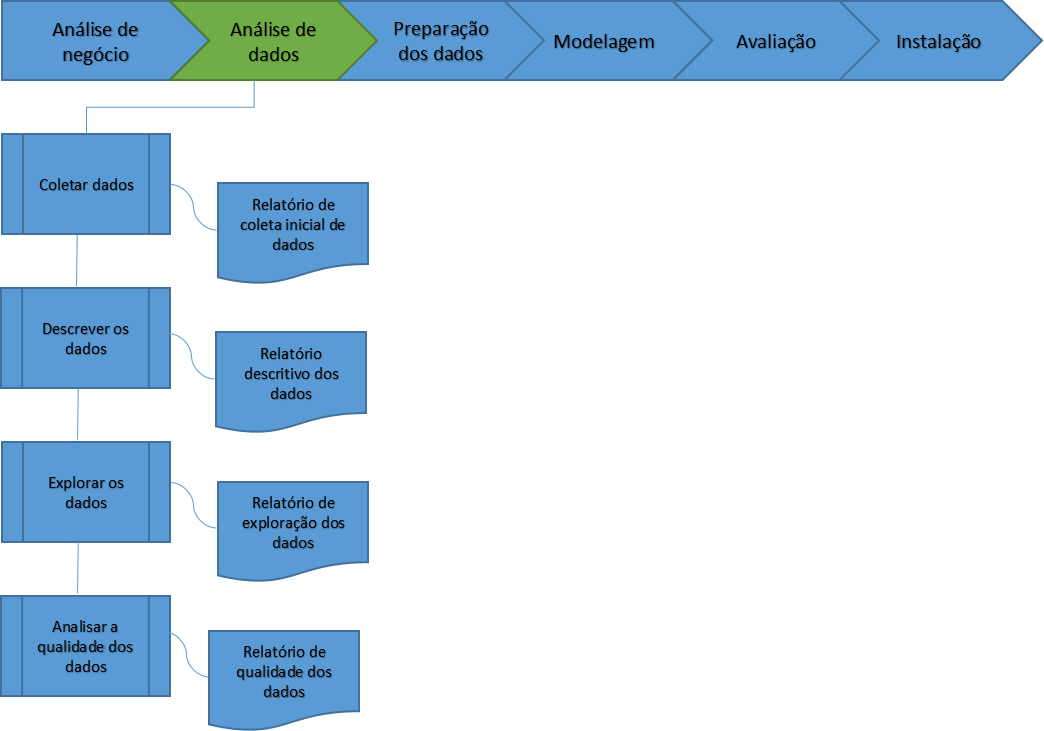
\includegraphics[scale=0.8]{img/CRISP-DM-Analise-dos-dados.png}
	\caption{Detalhamento da fase Análise de dados}
	\label{img:CRISP-DM-Analise-de-dados}
\end{figure}

% tarefas e saídas

\subsubsection*{\textbf{2.1 - Coletar dados}}

O objetivo desta tarefa é realizar a coleta dos dados indicados nos recursos do projeto. Nesta tarefa estão inclusos tanto o trabalho de extração quanto de integração dos dados, caso provenham de fontes diferentes, e carregamento dos dados em ferramenta específica, caso necessário.

\subsubsection*{Relatório inicial de coleta de dados}

Registra os conjuntos de dados coletados, suas localizações, os métodos utilizados na coleta e problemas, com respectivas soluções adotadas, que nela tenham ocorrido.

\subsubsection*{\textbf{2.2 - Descrever os dados}}

O objetivo desta tarefa é realizar uma análise estrutural dos dados, avaliando se eles satisfazem os requisitos do projeto.

\subsubsection*{Relatório descritivo dos dados}

Registra informações estruturais sobre os dados coletados, como formato, quantidade de registros e nomes de atributos.

\subsubsection*{\textbf{2.3 - Explorar os dados}}

O objetivo desta tarefa é realizar uma análise da distribuição dos dados, através de consultas, visualizações e técnicas de report\todo{qual a tradução para report techniques...}. Nela estão inclusas análise da distribuição de atributos dos dados, análise do relacionamento entre pares de atributos, análise de subpopulações e análise estatística. Essa análise serve tanto para suportar diretamente os objetivos de Mineração de Dados, quanto para refinar as informações sobre a estrutura e a qualidade dos dados.

\subsubsection*{Relatório de exploração dos dados}

Registra as informações descobertas na tarefa Explorar os dados e o impacto que poderão causar no projeto.

\subsubsection*{\textbf{2.4 - Analisar a qualidade dos dados}}

O objetivo desta tarefa é analisar a qualidade dos dados, verificando, por exemplo, se são completos(há registros para todos os casos necessários), se são corretos(frequência de erros), se há dados ausentes; e analisar soluções para os problemas de qualidade encontrados.

\subsubsection*{Relatório de qualidade dos dados}

Registra os resultados da análise de qualidade dos dados, indicando os problemas de qualidade e as possíveis soluções.

\newpage

\subsection*{3 - Preparação dos dados}

% diagrama

\begin{figure}[H]
	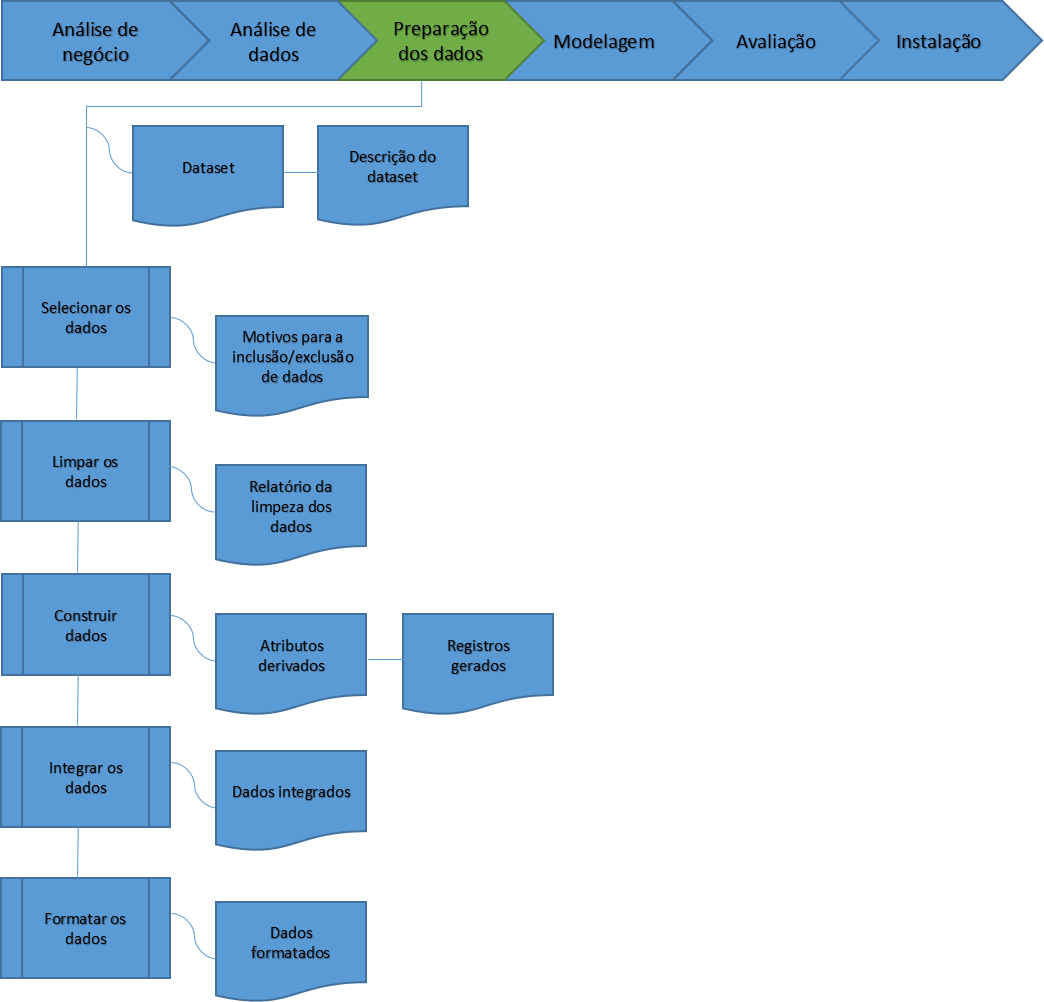
\includegraphics[scale=0.8]{img/CRISP-DM-Preparacao-dos-dados.png}
	\caption{Detalhamento da fase Preparação dos dados}
	\label{img:CRISP-DM-Preparacao-dos-dados}
\end{figure}

% tarefas e saídas

\subsubsection*{Datasets}

Datasets produzidos nesta fase, a serem utilizados no desenvolvimento de modelos ou em análises.

\subsubsection*{Descrição dos datasets}

Registra informações sobre os datasets produzido nesta fase.

\subsubsection*{\textbf{3.1 - Selecionar dados}}

O objetivo desta tarefa é selecionar datasets a serem utilizados em análises posteriores. Essa seleção envolve tanto a seleção de registros quanto a seleção de atributos. A lista de critérios para essa seleção inclui relevância dos dados para os objetivos de Mineração de Dados, qualidade e restrições técnicas, como limite no volume dos dados.

\subsubsection*{Motivos para inclusão/exclusão de dados}

Registra os motivos para inclusão e exclusão de dados realizadas na tarefa Selecionar dados.

\subsubsection*{\textbf{3.2 - Limpar os dados}}

O objetivo desta tarefa é produzir um dataset com nível de qualidade adequado para a aplicação das técnicas e modelos selecionados pelo projeto, resolvendo os problemas de qualidade analisados na tarefa Analisar a qualidade dos dados. Para tanto, atividades como seleção de subconjunto dos dados, inserção de valores padrão e estimação de valores ausentes poderão ser necessárias.

\subsubsection*{Relatório da limpeza dos dados}

Registra as alterações realizadas nos dados para resolver problemas de qualidade, indicando os motivos e possíveis consequências.

\subsubsection*{\textbf{3.3 - Construir dados}}

O objetivo desta tarefa é a criação de novos dados, através da derivação, a partir dos dados disponíveis, de novos registros ou atributos.

\subsubsection*{Atributos derivados}

Registra os atributos que foram construídos a partir de outros já existentes. Por exemplo, $área\ =\ altura \times largura$.

\subsubsection*{Registros gerados}

Registra os registros que foram construídos a partir de outros já existentes. \todo{pensar em exemplo de construção de registro} 

\subsubsection*{\textbf{3.4 - Integrar os dados}}

O objetivo desta tarefa é criar novos dados através da integração de dados de fontes diversas.

\subsubsection*{Dados integrados}

Dados resultantes da tarefa Integrar os dados, indicando quais fontes foram utilizadas e de que forma foi realizada a integração.

%%%%%%%%%%%%%%%%%%%%%%% parei aqui %%%%%%%%%%%%%%%%%%%%%%%%%%%%%%
\subsubsection*{\textbf{3.5 - Formatar os dados}}

O objetivo desta tarefa é realizar transformações nos dados que não alterem seus significados, necessárias para que os dados possam ser utilizados pelas ferramentas. Exemplos de transformações são mudança do formato do arquivo onde estão os dados, alteração na ordem das colunas ou alteração na ordem dos registros.

\subsubsection*{Dados formatados}

Registra as transformações realizadas nos dados, indicando motivos e possíveis consequências.

\newpage 

\subsection*{4 - Modelagem}

% diagrama

\begin{figure}[H]
	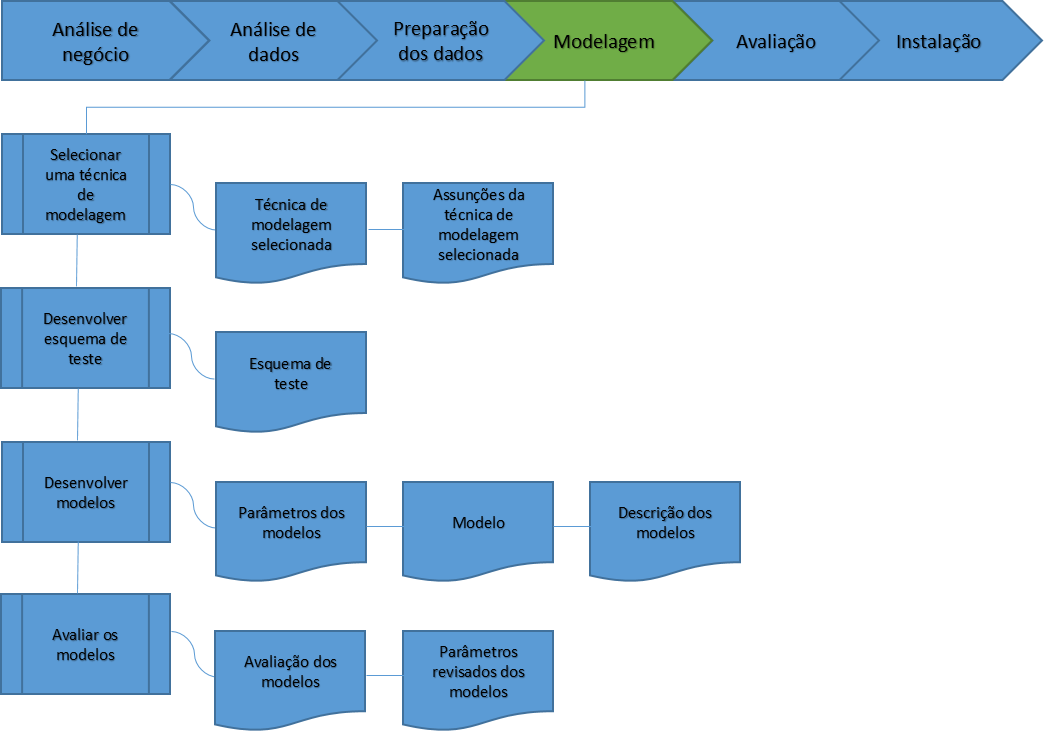
\includegraphics[scale=0.8]{img/CRISP-DM-Modelagem.png}
	\caption{Detalhamento da fase Modelagem}
	\label{img:CRISP-DM-Modelagem}
\end{figure}

% tarefas e saídas

\subsubsection*{\textbf{4.1 - Selecionar uma técnica de modelagem}}

O objetivo desta tarefa é selecionar uma técnica de modelagem a ser aplicada a um dataset gerado. No caso de várias técnicas de modelagem terem sido escolhidas para serem aplicadas, esta tarefa deve ser executada para cada uma delas.

\subsubsection*{Técnica de modelagem selecionada}

Registra informações sobre a técnica de modelagem selecionada.

\subsubsection*{Assunções da técnica de modelagem selecionada}

Registra as assunções feitas pela técnica de modelagem selecionada. Por exemplo, que todos os registros são independentes ou que todos os atributos possuem distribuição uniforme.

\subsubsection*{\textbf{4.2 - Desenvolver esquema de teste}}

O objetivo desta tarefa é desenvolver um procedimento ou mecanismo para testar a qualidade e validade do modelo a ser desenvolvido. Para tanto, deve-se decidir, por exemplo, sobre como os dados serão particionados em subconjuntos de treinamento e de teste e quais métricas serão utilizadas para avaliar o desempenho.

\subsubsection*{Esquema de teste}

Registra um plano para treinamento, teste e avaliação do modelo a ser desenvolvido.

\subsubsection*{\textbf{4.3 - Desenvolver modelos}}

O objetivo desta tarefa é aplicar a técnica de modelagem escolhida ao dataset desenvolvido na fase anterior.

\subsubsection*{Parâmetros dos modelos}

Registra os parâmetros utilizados pelos modelos desenvolvidos, bem como os motivos para suas escolhas.

\subsubsection*{Modelos}

Modelos desenvolvidos.

\subsubsection*{Descrição dos modelos}

Registra informações sobre os modelos desenvolvidos, como, por exemplo, como interpretá-los.

\subsubsection*{\textbf{4.4 - Avaliar os modelos}}

O objetivo desta tarefa é avaliar os modelos desenvolvidos sob uma perspectiva de Mineração de Dados, verificando se os critérios de sucesso de Mineração de Dados foram satisfeitos, se os resultados do testes foram satisfatórios. Os modelos desenvolvidos devem ser então comparados e ordenados de acordo com critérios de avaliação.

\subsubsection*{Avaliação dos modelos}

Registra os resultados da tarefa Avaliar o modelo, como a performance dos modelos desenvolvidos e uma ordem dos modelos de acordo com critérios de qualidade.

\subsubsection*{Parâmetros revisados dos modelos}

Registra alterações propostas em parâmetros dos modelos desenvolvidos de acordo com a avaliação dos modelos. Os parâmetros revisados servem para serem utilizados no desenvolvimento, em uma nova iteração, de novos modelos.

\newpage 

\subsection*{5 - Avaliação}

% diagrama

\begin{figure}[H]
	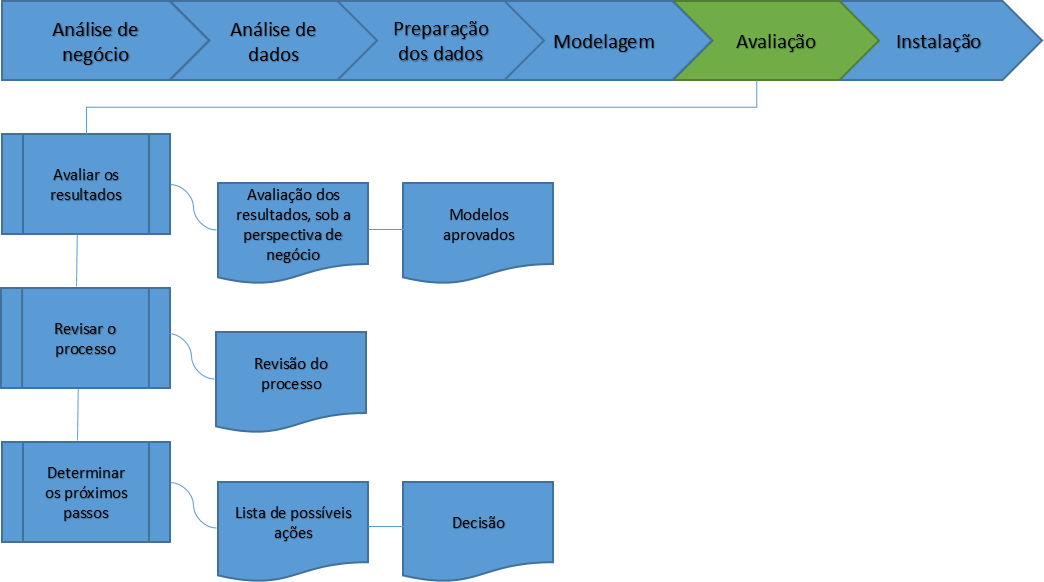
\includegraphics[scale=0.8]{img/CRISP-DM-Avaliacao.png}
	\caption{Detalhamento da fase Avaliação}
	\label{img:CRISP-DM-Avaliacao}
\end{figure}

% tarefas e saídas

\subsubsection*{\textbf{5.1 - Avaliar os resultados}}

O objetivo desta tarefa é avaliar em que medida os resultados alcançados com a Mineração de Dados, sejam modelos desenvolvidos, sejam informações extraídas, auxiliam no alcance dos objetivos de negócio e, se possível, testar os modelos desenvolvidos em aplicações reais.

\subsubsection*{Avaliação dos resultados, sob a perspectiva de negócio}

Registra a avaliação dos resultados, indicando se o projeto obteve sucesso em suportar os objetivos de negócio.

\subsubsection*{Modelos aprovados}

Conjunto de modelos que na avaliação dos resultados apresentaram resultados satisfatórios.

\subsubsection*{\textbf{5.2 - Revisar o processo}}

A partir deste ponto do processo os modelos desenvolvidos já apresentam resultados satisfatórios e torna-se apropriada a realização de uma revisão do processo, a fim de verificar a qualidade das atividades até então desenvolvidas.

\subsubsection*{Revisão do processo}

Registra os resultados da revisão do processo, indicando atividades que não foram desenvolvidas com a qualidade esperada e que deverão ser repetidas.

\subsubsection*{\textbf{5.3 - Determinar os próximos passos}}

O objetivo desta tarefa é definir quais as próximas atividades a serem desenvolvidas, de acordo com os resultados da avaliação dos resultados, da revisão do processo e dos recursos disponíveis para o projeto. Pode-se decidir pela implantação dos modelos desenvolvidos, pela realização de uma nova iteração ou a finalização do projeto.

\subsubsection*{Lista de possíveis ações}

Registra as potenciais ações a serem executadas e os respectivos motivos para execução ou não.

\subsubsection*{Decisão}

Registra a decisão sobre quais os próximos passos a serem seguidos e a respectiva motivação.

\newpage 

\subsection*{6 - Instalação}

% diagrama

\begin{figure}[H]
	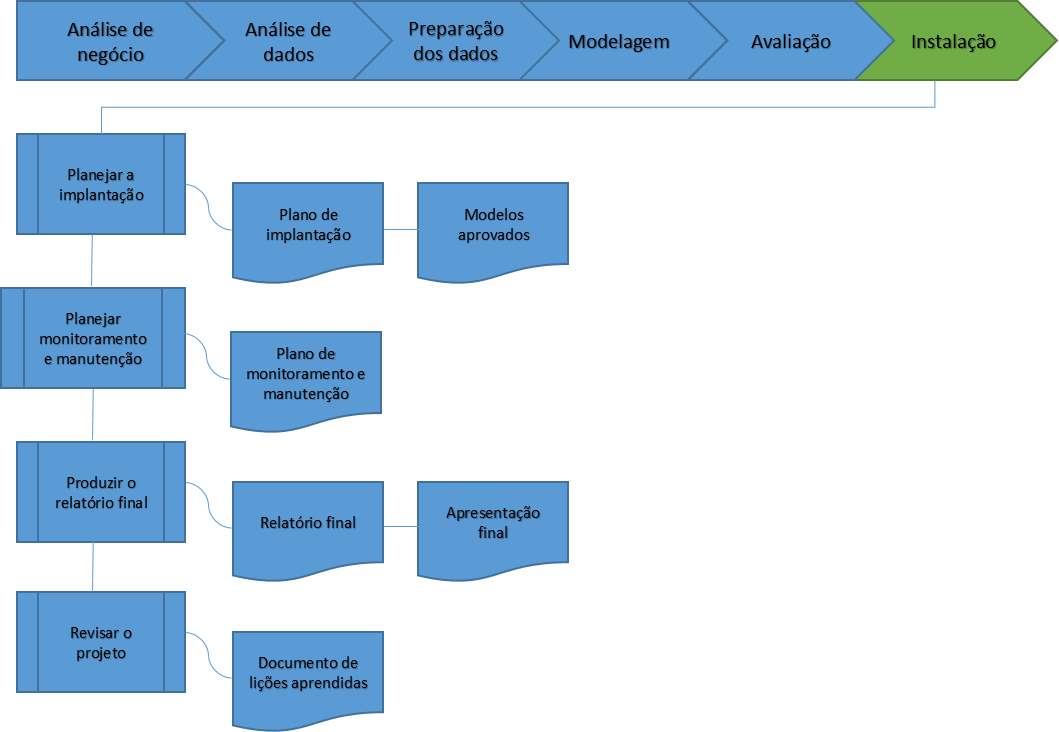
\includegraphics[scale=0.8]{img/CRISP-DM-Implantacao.png}
	\caption{Detalhamento da fase Implantação}
	\label{img:CRISP-DM-Implantação}
\end{figure}

% tarefas e saídas

\subsubsection*{\textbf{6.1 - Planejar a implantação}}

O objetivo desta tarefa é produzir um plano de implantação dos modelos aprovados.

\subsubsection*{Plano de implantação}

Registra as atividades necessárias para a implantação dos modelos aprovados.

\subsubsection*{\textbf{6.2 - Planejar monitoramento e manutenção}}

O objetivo desta tarefa é desenvolver planos de monitoramento e manutenção, objetivando verificar os resultados dos modelos implantados e evitar que sejam utilizados indevidamente ou tornem-se obsoletos.

\subsubsection*{Plano de monitoramento e manutenção}

Registra as estratégias de monitoramento e de manutenção.

\subsubsection*{\textbf{6.3 - Produzir relatório final}}

O objetivo desta tarefa é produzir um relatório registrando um histórico do projeto.

\subsubsection*{Relatório final}

Registra um histórico do projeto.

\subsubsection*{Apresentação final}

Apresentação dos resultados alcançados pelo projeto.

\subsubsection*{\textbf{6.4 - Revisar o projeto}}

O objetivo desta tarefa é analisar o que foi feito correta e incorretamente no projeto.

\subsubsection*{Documento de lições aprendidas}

Registra as lições aprendidas no projeto, indicando que ações foram executadas corretamente, para que sejam reforçadas, e que ações foram executadas incorretamente, para que sejam corrigidas em futuros projetos.

\section{Ferramentas utilizadas}

\cite{scikit-learn}
\cite{pandas}
%\chapter{Pontos de partida}

Como pontos de partida, consideraremos:

\begin{itemize}

\item Analisar o problema da predição de aluno com alta probabilidade de evasão do curso a partir de dados referentes a sua vida pré universidade e dados de seu desempenho no primeiro semestre do curso. Esse problema é relevante àqueles interessados na diminuição de taxas de evasão de cursos a partir de atividades voltada a discentes em grupo de risco de evasão.

\item Analisar o problema da predição do desempenho de um discente em uma disciplina a partir de dados sobre seu histórico como discente. Esse problema é relevante àqueles interessados na melhoria do desempenho de discentes em uma determinada disciplina a partir de atividades a serem iniciadas antes de o discente efetivamente cursá-la.

\item Analisar o problema da predição da taxa de evasão de um curso a partir de seus dados, como, por exemplo, de sua estrutura curricular. Esse problema é relevante ao processo de desenho ou redesenho de um curso, sua solução podendo ser utilizado como guia para decisões acerca do curso.

\end{itemize}


%\chapter{Resultados}
%\chapter{Conclusão}

% ---
% Finaliza a parte no bookmark do PDF, para que se inicie o bookmark na raiz
% ---
\bookmarksetup{startatroot}% 
% ---

% ----------------------------------------------------------
% ELEMENTOS PÓS-TEXTUAIS
% ----------------------------------------------------------
\postextual

% ----------------------------------------------------------
% Referências bibliográficas
% ----------------------------------------------------------

\bibliography{../referencias}
% ----------------------------------------------------------
% DEMAIS ELEMENTOS PÓS-TEXTUAIS
% ----------------------------------------------------------
% % ----------------------------------------------------------
% Glossário
% ----------------------------------------------------------
%
% Consulte o manual da classe abntex2 para orientações sobre o glossário.
%
%\glossary

% ----------------------------------------------------------
% Apêndices
% ----------------------------------------------------------

% ---
% Inicia os apêndices
% ---
\begin{apendicesenv}

% Imprime uma página indicando o início dos apêndices
\partapendices

% ----------------------------------------------------------
\chapter{Quisque libero justo}
% ----------------------------------------------------------

\lipsum[50]

% ----------------------------------------------------------
\chapter{Nullam elementum urna vel imperdiet sodales elit ipsum pharetra ligula
ac pretium ante justo a nulla curabitur tristique arcu eu metus}
% ----------------------------------------------------------
\lipsum[55-57]

\end{apendicesenv}
% ---


% ----------------------------------------------------------
% Anexos
% ----------------------------------------------------------

% ---
% Inicia os anexos
% ---
\begin{anexosenv}

% Imprime uma página indicando o início dos anexos
\partanexos

% ---
\chapter{Morbi ultrices rutrum lorem.}
% ---
\lipsum[30]

% ---
\chapter{Cras non urna sed feugiat cum sociis natoque penatibus et magnis dis
parturient montes nascetur ridiculus mus}
% ---

\lipsum[31]

% ---
\chapter{Fusce facilisis lacinia dui}
% ---

\lipsum[32]

\end{anexosenv}

%---------------------------------------------------------------------
% INDICE REMISSIVO
%---------------------------------------------------------------------

% \cleardoublepage
% \phantomsection 
\printindex

\end{document}